\documentclass[english,11pt,letterpaper,onecolumn]{scrartcl}

%\usepackage[utf8]{inputenc}
\usepackage{babel}
\usepackage{amsmath}
\usepackage{amsfonts}
\usepackage{mathptmx}
\usepackage{enumitem}
% Extra leading.
\renewcommand{\baselinestretch}{1.125}
\usepackage{tocloft}
% \usepackage{fancyhdr}
\usepackage{scrlayer-scrpage}
\usepackage{ifthen}
\usepackage{keyval}
\usepackage{geometry}
\usepackage{url}
\usepackage{calc}
\usepackage{array}
\usepackage{graphicx}
\usepackage{color}
\usepackage{listings}
\usepackage{supertabular}
%\usepackage{scrpage2}
\usepackage[pdftex,
colorlinks=true,
linkcolor=blue,
pdfpagelabels,
pdfstartpage=3
]{hyperref}
% \usepackage{poemscol}
% \global\verselinenumbersfalse
\makeindex
\definecolor{LstColor}{cmyk}{0.1,0.1,0,0.025} 
\setcounter{tocdepth}{9}
\newcommand\floor[1]{\lfloor#1\rfloor}
\newcommand\ceil[1]{\lceil#1\rceil}
\usepackage{lmodern}
\usepackage{amssymb,amsmath}
\usepackage{ifxetex,ifluatex}
\hypersetup{breaklinks=true,
    bookmarks=true,
    pdfauthor={},
    pdftitle={},
    colorlinks=true,
    citecolor=blue,
    urlcolor=blue,
    linkcolor=magenta,
    pdfborder={0 0 0}}

\usepackage{amsfonts}
\usepackage{amsmath}
\usepackage{amssymb}
\usepackage{graphicx}

\usepackage{version}%
\setcounter{MaxMatrixCols}{30}

%%%% Packages added - Peter
\usepackage{color}
\usepackage{amscd}     % commutative diagrams
\usepackage{mathrsfs}  % This package allows the use of script letters.
%%%%%%%%%%%%%%%%%%%%%%%%%%%%%%%%%%%%%%%%%%%%%%%%%%%%%

\newtheorem{theorem}{Theorem}[section]
%\theoremstyle{plain}
\newtheorem{acknowledgement}{Acknowledgement}
\newtheorem{algorithm}{Algorithm}[section]
\newtheorem{axiom}{Axiom}[section]
\newtheorem{case}{Case}[section]
\newtheorem{claim}{Claim}[section]
\newtheorem{conclusion}{Conclusion}[section]
\newtheorem{condition}{Condition}[section]
\newtheorem{conjecture}{Conjecture}[section]
\newtheorem{corollary}{Corollary}[section]
\newtheorem{criterion}{Criterion}[section]
\newtheorem{definition}{Definition}[section]
\newtheorem{example}{Example}[section]
\newtheorem{exercise}{Exercise}[section]
\newtheorem{lemma}{Lemma}[section]
\newtheorem{notation}{Notation}[section]
\newtheorem{problem}{Problem}[section]
\newtheorem{proposition}{Proposition}[section]
\newtheorem{remark}{Remark}[section]
\newtheorem{solution}{Solution}[section]
\newtheorem{summary}{Summary}[section]
\numberwithin{equation}{section}
\excludeversion{comment1}

%%%%% Macros added - Peter
\newcommand{\st}{\,|\,}
\newcommand{\C}{\mathbb{C}}
\newcommand{\F}{\mathbb{F}}
\newcommand{\I}{\mathbb{I}}
\newcommand{\bH}{\mathbb{H}}
\newcommand{\K}{\mathbb{K}}
\newcommand{\N}{\mathbb{N}}
\newcommand{\Q}{\mathbb{Q}}
\newcommand{\R}{\mathbb{R}}
\newcommand{\T}{\mathbb{T}}
\newcommand{\X}{\mathbb{X}}
\newcommand{\Y}{\mathbb{Y}}
\newcommand{\Z}{\mathbb{Z}}
%
\newcommand{\cB}{\mathcal{B}}
\newcommand{\cC}{\mathcal{C}}
\newcommand{\mcD}{\mathcal{D}}
\newcommand{\cE}{\mathcal{E}}
\newcommand{\cF}{\mathcal{F}}
\newcommand{\cG}{\mathcal{G}}
\newcommand{\calH}{\mathcal{H}}
\newcommand{\cJ}{\mathcal{J}}
\newcommand{\cK}{\mathcal{K}}
\newcommand{\mcL}{\mathcal{L}}
\newcommand{\cM}{\mathcal{M}}
\newcommand{\cN}{\mathcal{N}}
\newcommand{\cO}{\mathcal{O}}
\newcommand{\calR}{\mathcal{R}}
\newcommand{\cS}{\mathcal{S}}
\newcommand{\mcT}{\mathcal{T}}
\newcommand{\cU}{\mathcal{U}}
\newcommand{\cW}{\mathcal{W}}
\newcommand{\cY}{\mathcal{Y}}
\newcommand{\bcF}{\boldsymbol{\mathcal{F}}}
%
\newcommand{\oY}{\overline{Y}}
\newcommand{\uY}{\underline{Y}}
%
\renewcommand{\Re}{\mathop{\mathrm{Re}}}
\renewcommand{\Im}{\mathop{\mathrm{Im}}}
%
\newcommand{\card}{\mathop{\mathrm{card}}}
\newcommand{\Int}{\mathop{\mathrm{int}}}
\newcommand{\eps}{\varepsilon}
\newcommand{\kap}{\varkappa}
\newcommand{\be}{\begin{equation}}
\newcommand{\ee}{\end{equation}}
\newcommand{\inn}[2]{{\langle #1,#2 \rangle}}
\newcommand{\wt}[1]{{\widetilde{#1}}}

\newcommand{\conv}{\mathrm{conv}\,}
\newcommand{\bx}{{\boldsymbol{x}}}
\newcommand{\by}{{\boldsymbol{y}}}
\newcommand{\bk}{{\boldsymbol{k}}}
\newcommand{\bm}{{\boldsymbol{m}}}
\newcommand{\bc}{{\boldsymbol{c}}}
\newcommand{\ba}{{\boldsymbol{a}}}
\newcommand{\bp}{{\boldsymbol{p}}}
\newcommand{\bP}{{\mathbb{P}}}
\newcommand{\bS}{{\boldsymbol{S}}}
\newcommand{\bq}{{\boldsymbol{q}}}
\newcommand{\bfe}{{\boldsymbol{e}}}
\newcommand{\bone}{{\boldsymbol{1}}}
\newcommand{\bu}{{\boldsymbol{u}}}
\newcommand{\bv}{{\boldsymbol{v}}}
\newcommand{\bw}{{\boldsymbol{w}}}
\newcommand{\bff}{{\boldsymbol{f}}}
\newcommand{\bkk}{{\boldsymbol{k-1}}}
\newcommand{\bxi}{{\boldsymbol{Xi}}}
\newcommand{\balpha}{{\boldsymbol{\alpha}}}
\newcommand{\bbeta}{{\boldsymbol{\beta}}}
\newcommand{\bgamma}{{\boldsymbol{\gamma}}}
\newcommand{\blambda}{{\boldsymbol{\lambda}}}
\newcommand{\bmu}{{\boldsymbol{\mu}}}
\newcommand{\gr}{{\mathrm{graph\,}}}
\newcommand{\of}{\overline{f}}
\newcommand{\og}{\overline{g}}
\newcommand{\oc}{\overline{c}}
\newcommand{\ou}{\overline{u}}
\newcommand{\ox}{\overline{x}}
\newcommand{\oX}{\overline{X}}
\newcommand{\oXi}{\overline{X}_i}
\newcommand{\uc}{\underline{c}}
\newcommand{\oy}{\overline{y}}
\newcommand{\uy}{\underline{y}}
\newcommand{\odelta}{\overline{\delta}}
\newcommand{\udelta}{\underline{\delta}}
\newcommand{\oPhi}{\overline{\Phi}}
\newcommand{\map}{\textrm{Map}\,}
\newcommand{\loc}{\mathrm{loc}}
\newcommand{\mydot}{\;\cdot\;}
\DeclareMathOperator{\dom}{dom}
\DeclareMathOperator{\range}{range}
\DeclareMathOperator{\id}{id}
\DeclareMathOperator{\Aff}{Aff}
\DeclareMathOperator{\GL}{GL}
\DeclareMathOperator{\diag}{diag}

\usepackage[
backend=biber,
style=numeric,
sorting=ynt,
hyperref=true,
backref=true
]{biblatex}

\addbibresource{gogins.bib}
\begin{document}
    
    \title{Parametric Composition of Score Graphs}
    \author{Michael Gogins \\ \texttt{michael.gogins@gmail.com}}
    \maketitle
    %\pagestyle{scrheadings}
    
    %\lohead{Parametric Composition}
    
    \section{Introduction}
    
    We define a \textit{score space} as a space in which a set of points 
represents 
    a piece of music, \textit{e.g.} notes on the grand staff, punches in a 
piano 
    roll, some more abstract space, or even grains of sound on a sonogram. We 
    define a \textit{score generator} as a computer program that generates a 
    musical score in some score space. We define a \textit{parametric score 
        generator} as one whose behavior is completely defined by numerical 
    parameters. 
    
    Then \textit{parametric composition} is the art of composing music by 
exploring 
    the parameter space of some parametric score generator. Such exploration 
can be 
    performed by literally zooming around in a colored map of the parameter 
space, 
    by interpolating between two parameter points in that space, or by 
evolving 
    parameters using the genetic algorithm. 
    
    Parametric composition has previously been investigated with respect to 
the 
    generation of pieces in spaces that directly represent either sound, 
    \textit{e.g.} in the form of a grid of sound grains (Gabor transform) 
    \cite{obsessed}, or scores, \textit{e.g.} in the form of a grid of notes 
(piano 
    roll) \cite{ifsmusic}. Here, pieces are generated in a score space 
constructed 
    from the basic symmetries of chord space identified by Callender, Quinn 
and 
    Tymoczko \cite{callender:346}, along with revoicings and rearrangements. 
The 
    dimensions of this score space are: set class (the most basic form of a 
chord) 
    $P$ (\textit{i.e.}, Callender \textit{et al.}'s $OPTIC$), inversion $I$, 
    transposition $T$, octavewise revoicings $v$, and rearrangements of voices 
$a$. 
    In $PITva$ space, a piece of note-based music may be considered a 
succession of 
    more or less fleeting chord points or, in other words, as the graph of a 
    vector-valued function of time in the score space, which we call a 
    \textit{score graph} of a \textit{score function},
    
    $$(P, I, T, v, a) = r(t).$$ 
    
    \noindent The notes and chords do \textit{not} need to be confined to 
12-tone 
    equal temperament. One motivation for using score functions to compose is 
that, 
    at any one point in time, there is one and only one ``harmony.''
    
    The score generators used here are \textit{iterated function systems} 
(IFSs) 
    \cite{barnsley1985iterated, 10.2307/24893080, fractalseverywhere}. More 
    particularly, our score generators are special IFSs where the contractive 
    transformations that make up the IFS are constrained such that the IFS 
computes 
    not any old attractors, but only attractors that closely approximate the 
graphs 
    of functions. These are called \textit{fractal approximations} (FAs) or 
fractal 
    interpolations \cite{Barnsley1986, fractalseverywhere, 
navascues2014fractal}. 
    The function for such a graph is called simply a \textit{fractal function}. 
It 
    is interesting that all continuous functions are fractal functions 
    \cite{2016arXiv161001369B}. Even more particularly, we use FAs to compute 
    graphs of $r$. The advantage of such FAs is that \textit{any} score can be 
so 
    generated, and \textit{every} FA of this type generates a graph of some 
$r$.
    
    A FA may be completely specified as a set of numerical parameters. Thus, 
any 
    piece of note-based music may be approximated as closely as desired by a 
fixed 
    size set of numerical parameters.
    
    Although there might be dozens or hundreds of numbers in such FA 
parameters, 
    each parameter set can effectively be represented as a single real or 
complex 
    number by using a recursive indexing scheme such as a Hilbert index 
    \cite{hamilton2006compact}. We call this number the \textit{effective 
        parameter} of the FA because the complete set of parameters, can be 
    recovered (given sufficient numerical precision) by decoding the index. 
    
    Then, using the effective parameters, it is simple to compute a parametric 
map 
    of all pieces within a given range of FAs, or to interpolate between two 
pieces 
    by interpolating between their effective parameters. It is also, of 
course, 
    possible to evolve pieces using the genetic algorithm on sets of actual 
    parameters.
    
    The remainder of this paper develops the mathematical background in 
somewhat 
    more detail; discusses the implementation of fractels, fractal 
approximations, 
    Hilbert indices, and the genetic algorithm for FA parameters in the 
Silencio 
    library for algorithmic composition in JavaScript; and finishes with 
examples 
    of each of the three methods of algorithmic composition, implemented in 
    Silencio and Csound.
    
    \section{Mathematical Development}
    
    This section is not intended as a complete, self-contained exposition but 
    rather as providing entry points for readers who have some exposure to 
    mathematical music theory or fractal geometry. I have tried to supply 
    references not only to original publications of ideas, but also to recent 
    reviews or summaries.
    
    TO DO: Really understand (a) what is a local IFS, (b) how exactly does the 
RB 
    operator compute one, and what this all has to do with fractels. What 
    \textit{is\textbf{}} clear is that they are trying specifically to produce 
IFS 
    whose attractors are graphs of functions.
    
    An RB operator is a kind of IFS in which the graph of a function over a 
segment 
    $[a, b]$ is approximated by mapping the $[a, b]$ to each of the 
sub-segments 
    defined by a pair of interpolation points.
    
    A \textit{local} IFS is one in which each function or mapping in the IFS 
may 
    have a different domain.
    
    Numerous maps can be used to construct an RB operator for a given graph. 
Here, 
    we use local iterated functions 
    instead of plain linear mappings for each interpolation segment.
    
    \subsection{Chord Spaces}
    
    A \textit{chord space} is simply a space in which each voice of a chord is 
    represented by a different dimension. A single voice is represented by a 
point 
    on a line; an interval, by a point on a plane; a triad, by a point in a 
    3-dimensional space; and so on. Here the octave is always 12, so that 
    pitch-classes in 12 TET are always integers (and compatible with MIDI). 
Chord 
    space has many uses. For example, Tymoczko \cite{tymoczko2006geometry, 
        tymoczko2011geometry} showed that perceptually smoother voice-leadings 
between 
    chords are represented by shorter distances in chord space. 
    
    Even unschooled musicians are aware that pitches transposed to different 
    octaves are somehow the same. This is expressed in music theory by saying 
that 
    pitch-classes, \textit{e.g.} C or F\#, are pitches under \textit{octave 
        equivalence}. Octave equivalence transforms the line of pitch into a 
circle, 
    an \textit{orbifold} or \textit{quotient space} $\mathbb{R}/12$, by gluing 
the 
    lowest pitch under octave equivalence to the same pitch an octave higher. 
There 
    are other implicitly familiar equivalence classes in music: 
    \textit{permutational equivalence} (a triad is somehow the same whether 
the 
    voices are assigned to violin, trumpet, and flute or to flute, trumpet, 
and 
    violin), \textit{cardinality equivalence} (a chord is somehow the same if 
    voices are doubled in different octaves), and so on. Callender, Quinn, and 
    Tymoczko \cite{callender:346} have concisely analyzed these equivalence 
    classes, or symmetries, as different quotients of chord space. Figure 
    \ref{fig:opc} shows their $OPC$ orbifold  
    $\left(\mathbb{R}/12\mathbb{Z}\right)^{n}/\mathcal{S}_{n}$ (octave, 
    permutational, and cardinality equivalence) for trichords in 12-tone equal 
    temperament. In all cases $n$ is the the number of voices, and 
$\mathcal{S}$ 
    is the symmetry group. $OPC$ is what musicians commonly mean by ``chord.''
    
    \begin{figure}
        \centerline{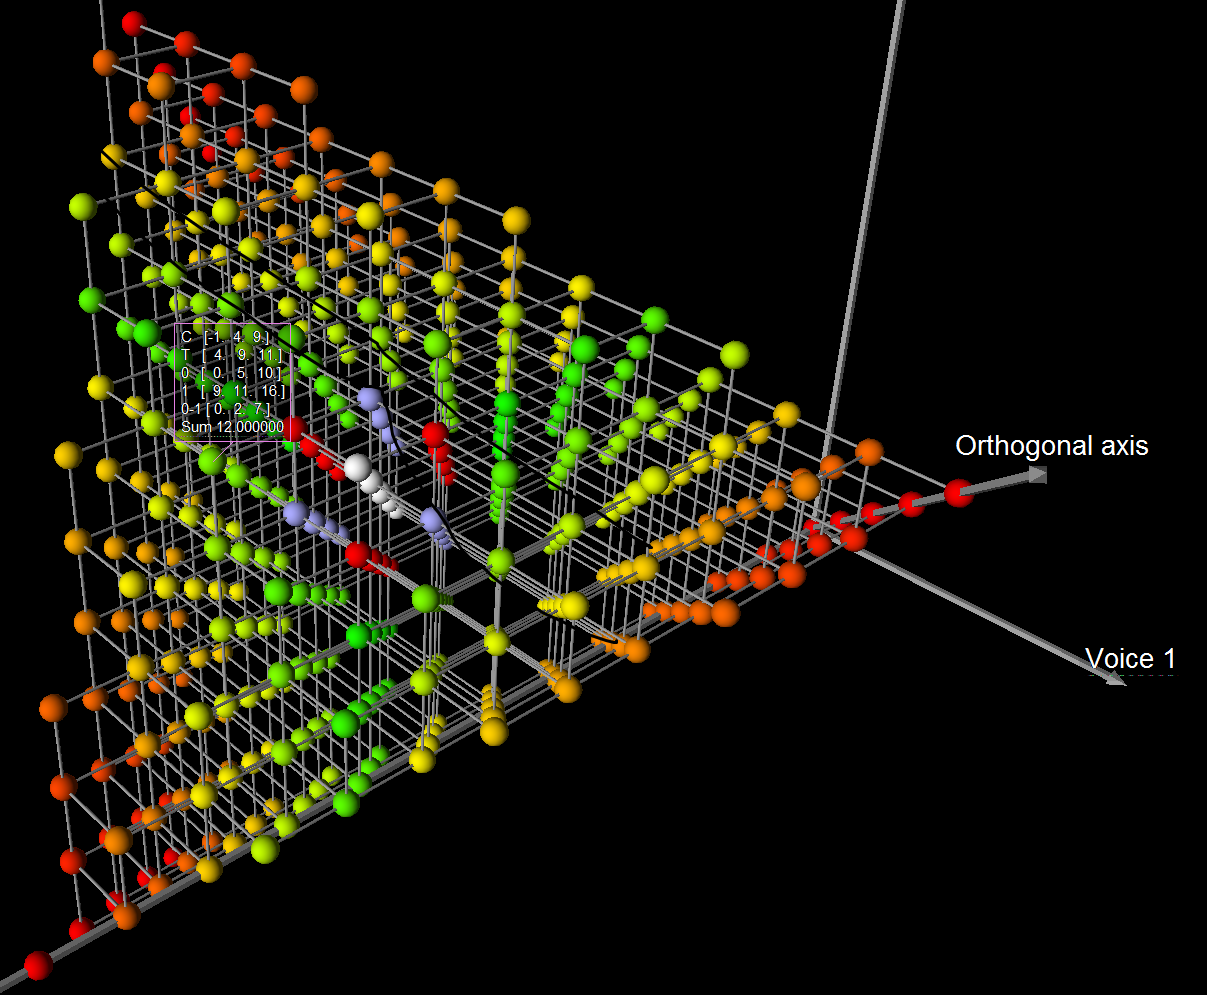
\includegraphics[width = 0.9\textwidth]{opc}}
        \caption{\label{fig:opc} 
            $OPC$ for trichords in 12TET.}
    \end{figure}
    
    If in addition transpositional equivalence is assumed, the orbifold 
collapses 
    to a single layer 
$\left(\mathbb{R}/12\mathbb{Z}\right)^{n-1}/\mathcal{S}_{n}$, 
    in which points at 120 degrees rotation are equivalent (Figure 
\ref{fig:optc}; 
    to simplify the view, pitches are rounded by semitone). This is $OPTC$, 
which 
    is what musicians normally mean by ``chord type.''
    
    \begin{figure}
        \centerline{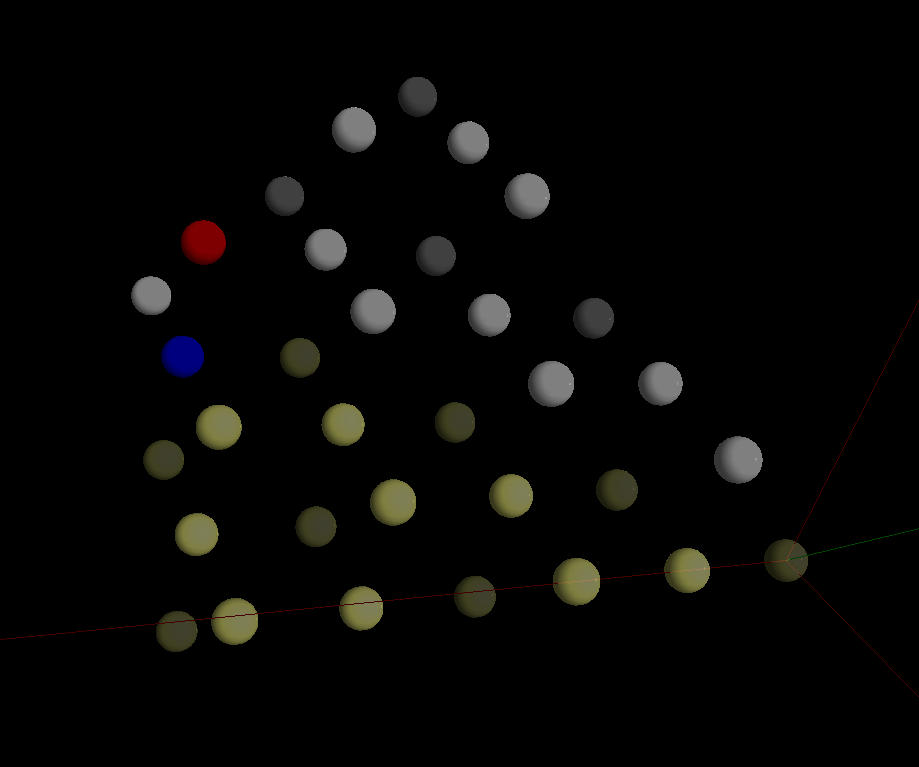
\includegraphics[width = 0.9\textwidth]{opttc}}
        \caption{\label{fig:opttc} 
            $OPTC$ for trichords in 12TET.}
    \end{figure}
    
    A little more theoretical sophistication reveals \textit{inversional 
        equivalence}: a major triad is somehow the same as a minor triad. The 
    orbifold folds over or reflects to equate major and minor 
    $\left(\mathbb{R}/12\mathbb{Z}\right)^{n-1}/(\mathcal{S}_{n} \times 
    \mathbb{Z}_{2})$ (Figure \ref{fig:optic}; again, rounded by semitone). This 
is 
    $OPTIC$, which is what theorists mean by ``set class,'' and is the most 
    abstract commonly used concept of what is a ``chord.''
    
    \begin{figure}
        \centerline{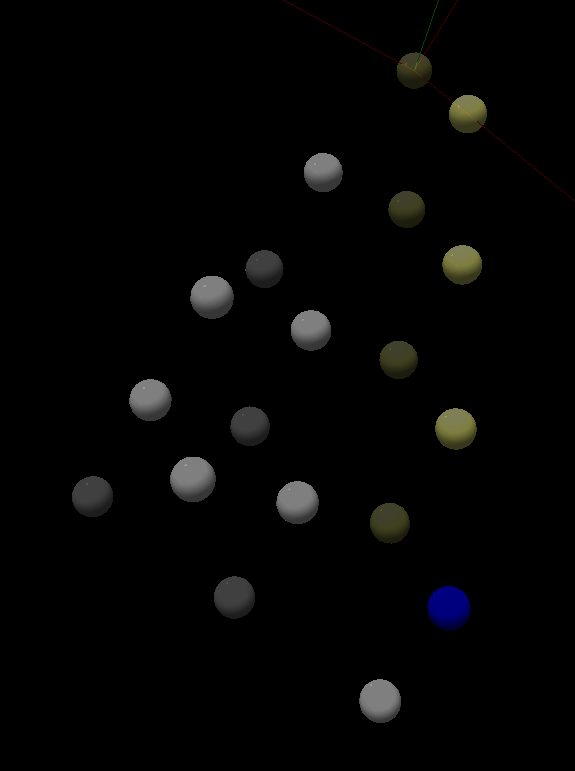
\includegraphics[width = 0.9\textwidth]{opttic}}
        \caption{\label{fig:optic} 
            $OPTIC$ for trichords in 12TET.}
    \end{figure}
    
    Here, we do not use chord space for composing. Rather, we construct a 
parameter 
    space in which each of the irreducible symmetries of chord space identified 
by 
    Callender, Quinn, and Tymoczko is a separate dimension, on which operations 
are 
    indexed. These are:
    
    \begin{enumerate}
        \item $P$ (Callender, Quinn, and Tymoczko's $OPTIC$ space) -- Set 
class, the 
        most abstract conception of a chord; all major and minor triads are 
equivalent. 
        The number of elements in P depends upon the maximum number of voices 
and the 
        number of divisions of the octave.
        \item $I$ -- Inversion.
        \item $T/R$ -- Transposition within a specified range $R$.
    \end{enumerate}
    
    \noindent To these we add:
    
    \begin{enumerate}[resume]
        \item $v$ -- octavewise revoicing (within some specified range) of the 
        $PIT$ chord, through all permutations of the possible voicings.
        \item $a$ -- Voicewise re-arrangement of voices or instrument, through 
all
        permutations of the possible arrangements.
    \end{enumerate}
    
    \noindent Obviously not all dimensions of this odd parameter space are 
    continuous. The purpose of $PITva$ space is to permit composing by moving 
a 
    single point through the space and thus controlling at once set class, 
    inversion, transposition, voicing, and arrangement; another way of saying 
this 
    is that any piece of note-based music can be represented by the 
    graph of a vector-valued function of time, $$(P, I, T, v, a) = 
    r(t).$$
    
    By assigning each symmetry to an orthogonal dimension of the $PITva$ space, 
the 
    IFSs to be developed for composing can more easily be adapted to control 
the 
    dimensions independently, \textit{e.g.}\ by generating arpeggiations 
without 
    affecting chord type.
    
    \subsection{Fractal Approximation}
    
    A fractal is simply a set of points that fills some definite fraction of 
its 
    space. A line on the plane occupies no space. A snowflake curve iterates 
    bending segments of the curve to infinity, and thus comes to occupy some 
    fraction of the plane \cite{Mandelbrot:1982:FGN}.
    
    One basic way to generate fractals is with the multiple copy reduction 
    machine (MCRM). Imagine a copier with more than one lens, each equipped 
with 
    adjustments (sliding, shrinking, or rotating the image of the original). 
Make 
    a copy, replace the original with the copy, and repeat to infinity. Just 
as 
    with the snowflake curve, the final copy comes to occupy a definite 
fraction 
    of the picture plane and thus is a fractal \cite{chaosandfractals}. 
    
    Mathematically, the MCRM is an iterated function system (IFS). Each lens 
    represents an affine transformation of the plane. Each lens, chosen at 
random 
    or in turns, transforms the original set, and the union of the 
transformations  
    replaces the original.
    
    An \emph{iterated function system (IFS)} is a topological space $X$
    together with a finite set of continuous functions $f_{n}:X\rightarrow X$, 
    $n=1,2,\dots,N$.
    
    If the transformations are contractive, the Banach Fixed Point Theorem 
proves 
    that iterating this process to infinity brings the original to a fixed 
point, 
    the attractor of the IFS \cite{chaosandfractals, barnsley1985iterated, 
        10.2307/24893080, fractalseverywhere}. \textit{Any} original will end 
up 
    producing the \textit{same} attractor. 
    
    An \emph{attractor} of the IFS $\mathcal{F}$ is a set
    $A\in H(X)$ such that
    
    \begin{enumerate}
        \item $\cF(A)=A$, and
        
        \item there is an open set $U\subset X$ such that $A\subset U$ and
        $\lim_{k\rightarrow\infty}\cF^{k}(S)=A,$ for all $S\in H$ with 
$S\subset U$,
        where the limit is with respect to the Hausdorff metric on $H$.
    \end{enumerate}
    
    
    Furthermore, Barnsley's Collage Theorem \cite{barnsley:1986:solution} 
proves 
    that any original set can be approximated, as closely as desired, by some 
IFS. 
    This is done by arranging the affine transformations to cover the original 
set 
    with transformed copies of itself, minimizing overlaps. \textit{The 
Collage 
        Theorem is the key motivation for using IFS in algorithmic music 
composition}: 
    IFS are simple yet extremely powerful. 
    
    The remainder of this paper concerns how to control this power: how to 
    filter out as many of the musically useless productions, which of course 
are 
    overwhelmingly more numerous, as possible; and how to explore the 
    remaining vast parameter space of IFS in a \textit{musical} way.
    
    It would be possible to use IFS to generate sound grains on a grid; to 
    generate notes on a grid; or to generate a path through a different chord 
    space, \textit{e.g.} use Callender, Quinn, and Tymoczko's OPC $\times$ 
    revoicings 
    $\times$ rearrangements instead of $PITva$. Again, the purpose is to 
filter 
    out unmusical productions. Since by the Collage Theorem IFSs are universal, 
we 
    cannot exclude such productions; but we can simply make it harder, take 
more 
    steps, to generate then. This is not an esthetic judgement. We are 
    simply trying to make the generative space more like the space of human 
    musical perception, as its geometry is implied by music theory.
    
    So, we have a piece as a sequence of points in $PITva$ space, or, 
    alternatively, the graph of a function of time in that space. IFSs can 
    be used to approximate graphs of functions by applying the Collage Theorem 
    as follows. This applies in spaces of any dimension, \textit{i.e.}\ to 
    vector-valued as 
    well as to single-valued functions:
    
    \begin{enumerate}
        \item Define the domain of the function, an interval $[a, b]$.
        \item Identify a set of interpolation points, samples of the value of 
the 
        function, within $[a, b]$, 
    \end{enumerate}
    
    
    
    
    
    
    
    
    
    
    \subsection{Hilbert Indices for Fractal Approximation Parameters}
    
    \section{Implementation Notes}
    
    \section{Musical Examples}
    
    \subsection{Parametric Mapping}
    
    
    \subsection{Interpolating Between Pieces}
    
    
    \subsection{Using the Genetic Algorithm with Fractal Interpolation 
Functions}
    
    \section{Future Directions}
    
    It is interesting that, as Massopust notes \cite{massopust2017}, 
    \begin{quote}D. Hardin proved in 2012 that every compactly supported 
        refinable function is a piecewise fractal function. In particular, the 
unique 
        compactly supported continuous function determined by the mask of a 
convergent 
        subdivision scheme is a piecewise fractal function. \end{quote} 
    This implies that the same technique of parametric 
    composition based on FAs and described here, would also work for composing 
    sound directly using refinable sets of sound grains, \textit{e.g.} 
wavelets.
    
    It also is interesting that Barnsley, Hegland, and Massopust 
    \cite{2013arXiv1309.0972B} discuss how to derive fractal approximations of 
    existing data sets. This implies that it is possible to automatically 
derive 
    FA parameters for existing works of note-based music, and then to use the 
    resulting parameter map or parametric interpolation to analyze the 
    relationship between the works, or to compose new works intermediate in 
form 
    between them.
    
    % \bibliographystyle{ieeetr}
    %\bibliographystyle{ieeetr}
    %\bibliography{gogins}{}
    \printbibliography
    
\end{document} 